%---Linda

\subsection{Methods}

Regarding to results of the previous years, it is given that the glacier velocity for the glaciers Tellbreen and Blekumbreen is less then one meter.
The general used GPS system has only an accurancy in the order of meters (cite).
This is the reason why we use the differential GPS, which gives a higher accurancy.
By correcting the raw data with the data from the base station, it is posssible to increase the accurancy to the order of millimeters.
The accurancy depends on the distance to the base station (Gölles, 2012) and differs between the horizontal and the vertical component.
The coordinates of the base station ar well known. 
So the disturbances by the atmosphere during the measuring time can be corrected. 
While the post processing the measured coordinates are compare on every timestep defined by the GPS time.
The effect on two measurements at the same postion on two different days are disscussed in the result section.\medskip

The GPS measurements have been done with the Trimble differential Global Navigation Satellite System (GNSS). 
The measured parameters were the northing and easting component as well as the elevation.
The setting during our measurements inculded the receiver Trimble R4, the controller Trimble TCS2 and a carbon pole to mount the receiver proberly next to the stake (see figure).\medskip

During the operation of the measuremts we followed exact the description in section 2 and 3 in Gölles (2012). 
The recommended Fast Static survey method is used.
The used coordinate system is the Universal Transversal Mercator (UTM) for the zone 33x with WGS 1984 date. 
The duration for our measurments with the GPS receiver was at least 15 minutes. 
We had to made choice with a trade off between the quality of the result and the total number of measurements to measure all stakes at least one time. 


\subsection{Setup}

The setup for our measurments is specifed by different guidelines to insure that the measurements are consistent during the whole fieldwork.
The rover on the carbon pole has to be positioned on the top on the stake as far as possible. 
To determine the error from a tilted stake, it is necessary to measure the inclination of the stake as well as the direction of iinclination with the compass.
The snow depth is measured with the probe.
With snow depth and the antenna height the actual elevation on the ice surface is known. 
In addition, the height from the rover above the ice surface is needed to calculate the error by the inclination of the stake.
When the stake is already melted out too high, it is possible to put the pole next to the stake. 
In this case the poles has to be northwards of the stake so that the correction is correlated to only to the northing component. 
Also the distance from rover pole to stake is measured.
For the height and distance measurements the accurancy is one centimeter, because of the one centimeter scale.
The measurement of the inlination with compass has accurancy of two degree caused by the two degree scale.

\begin{figure}
\centering
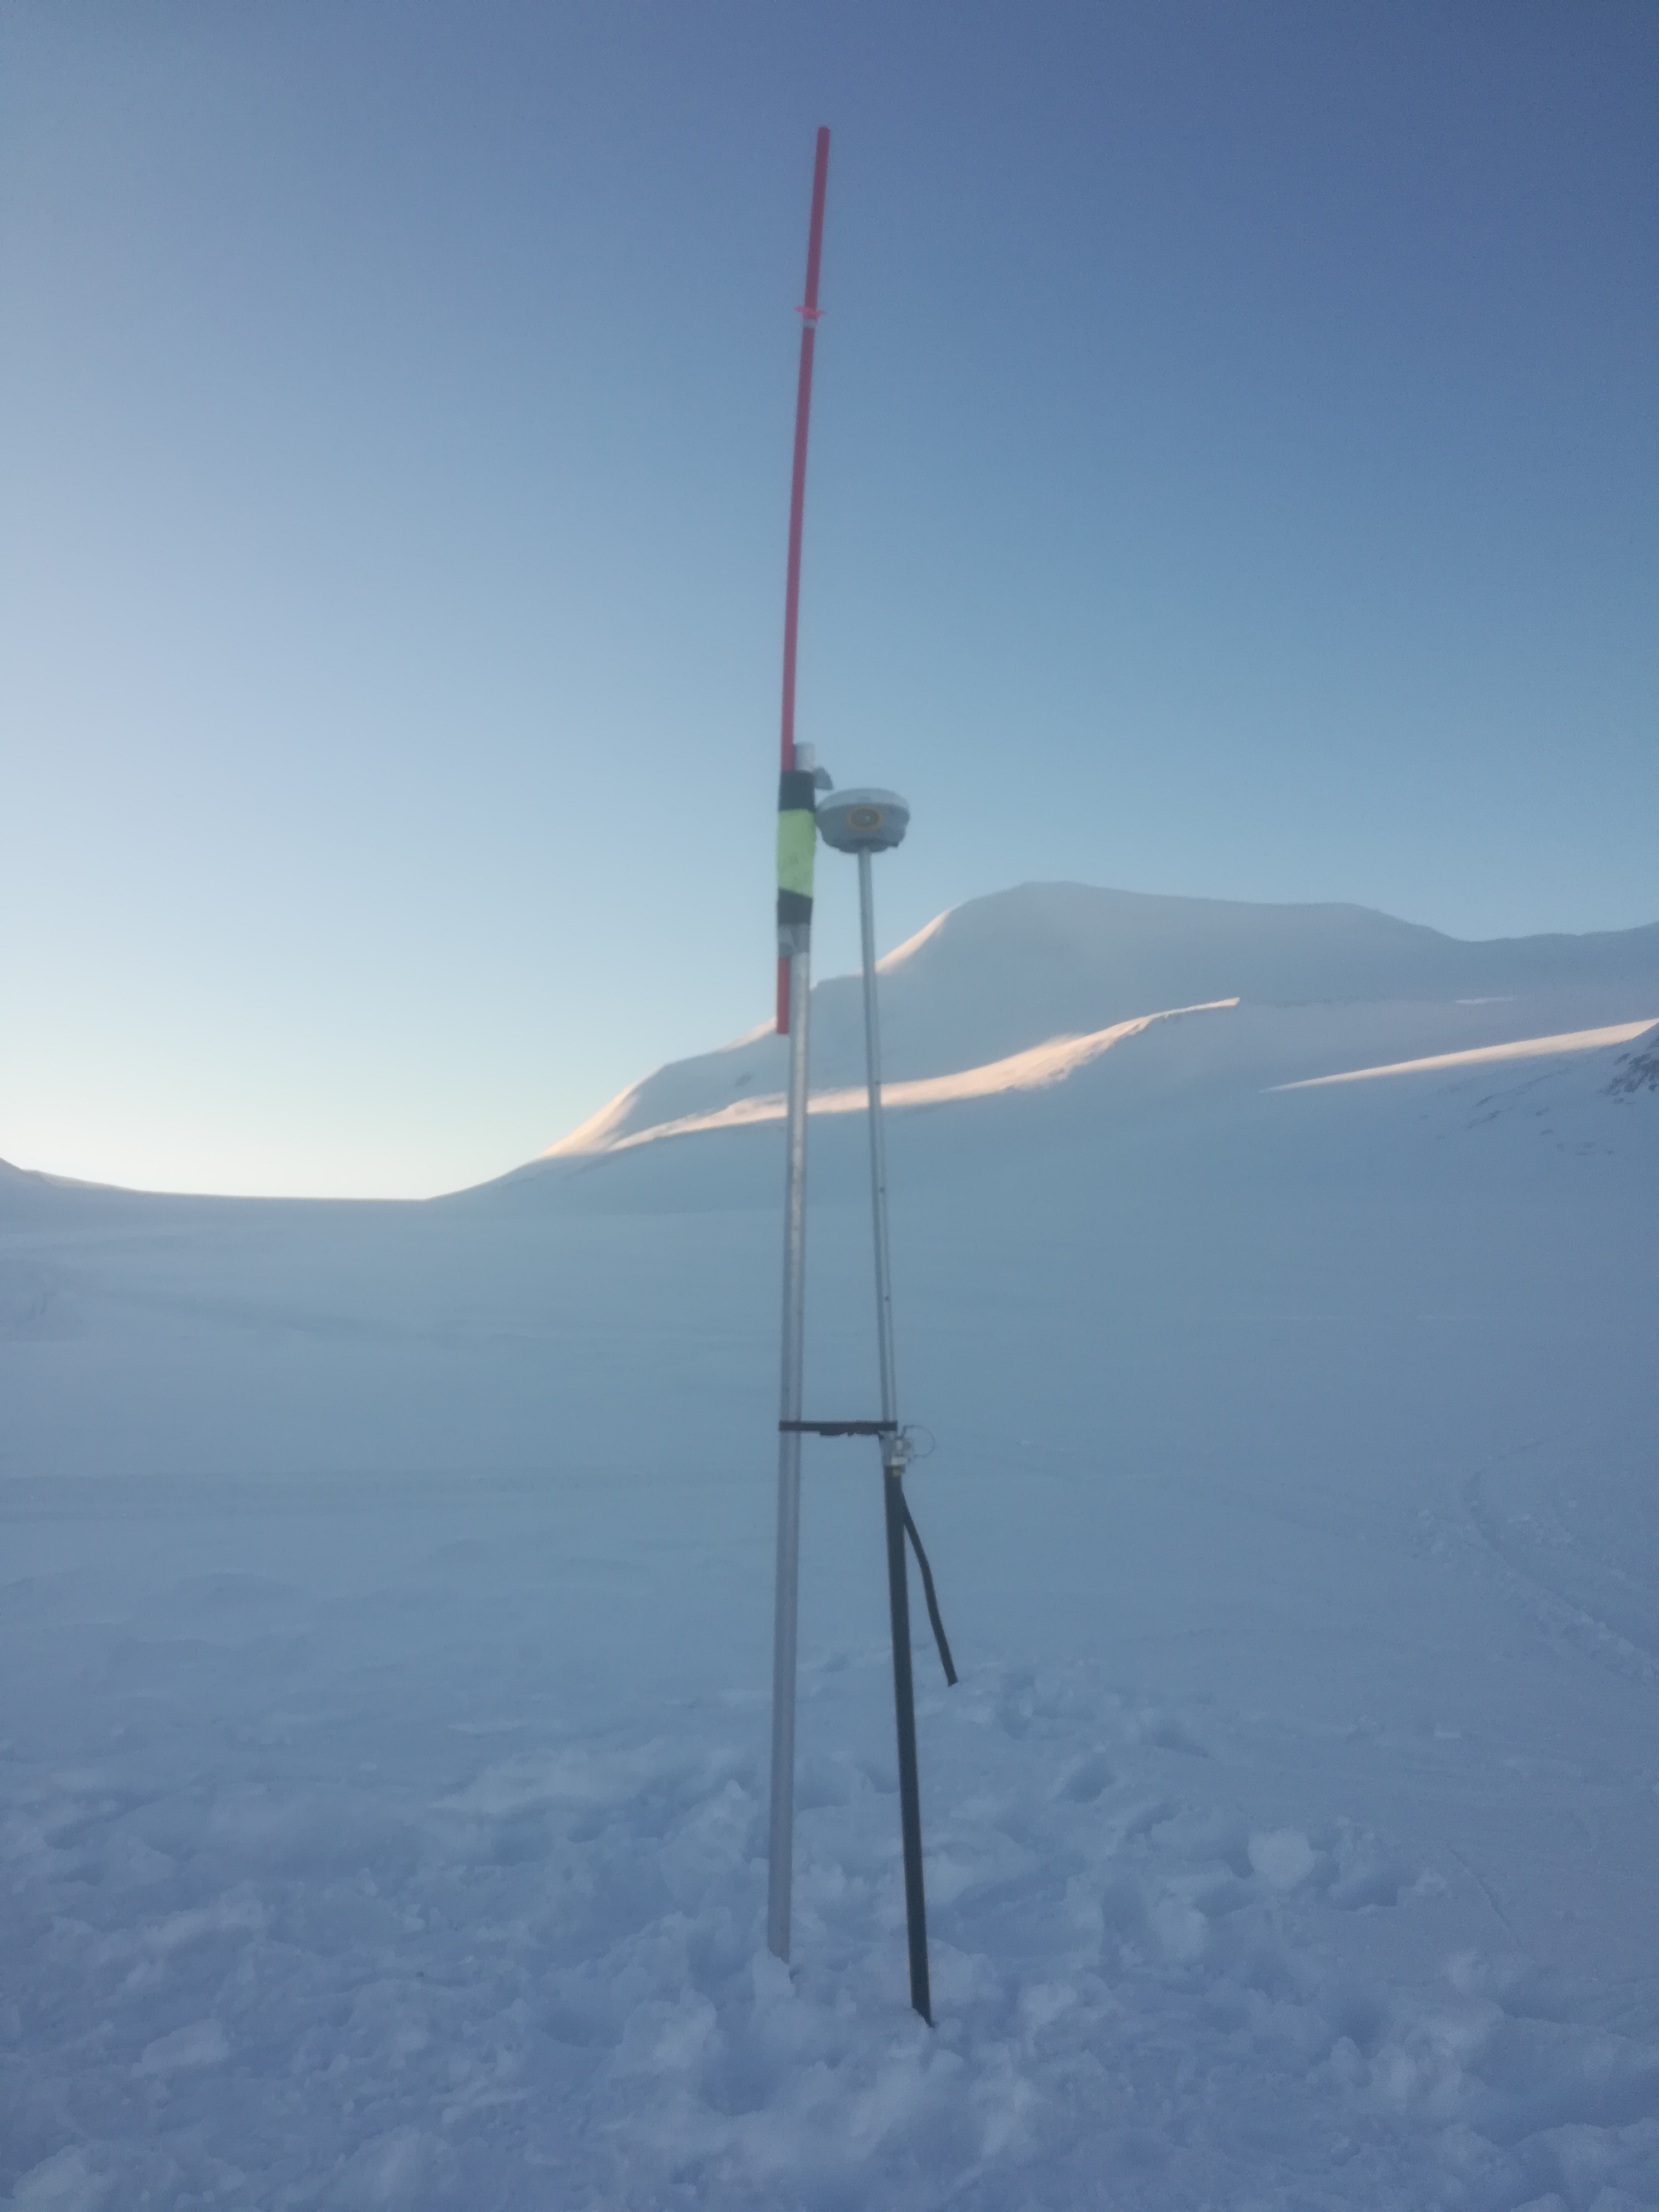
\includegraphics[width=0.48\linewidth]{/figs/pictures/GPS_setup.jpg}
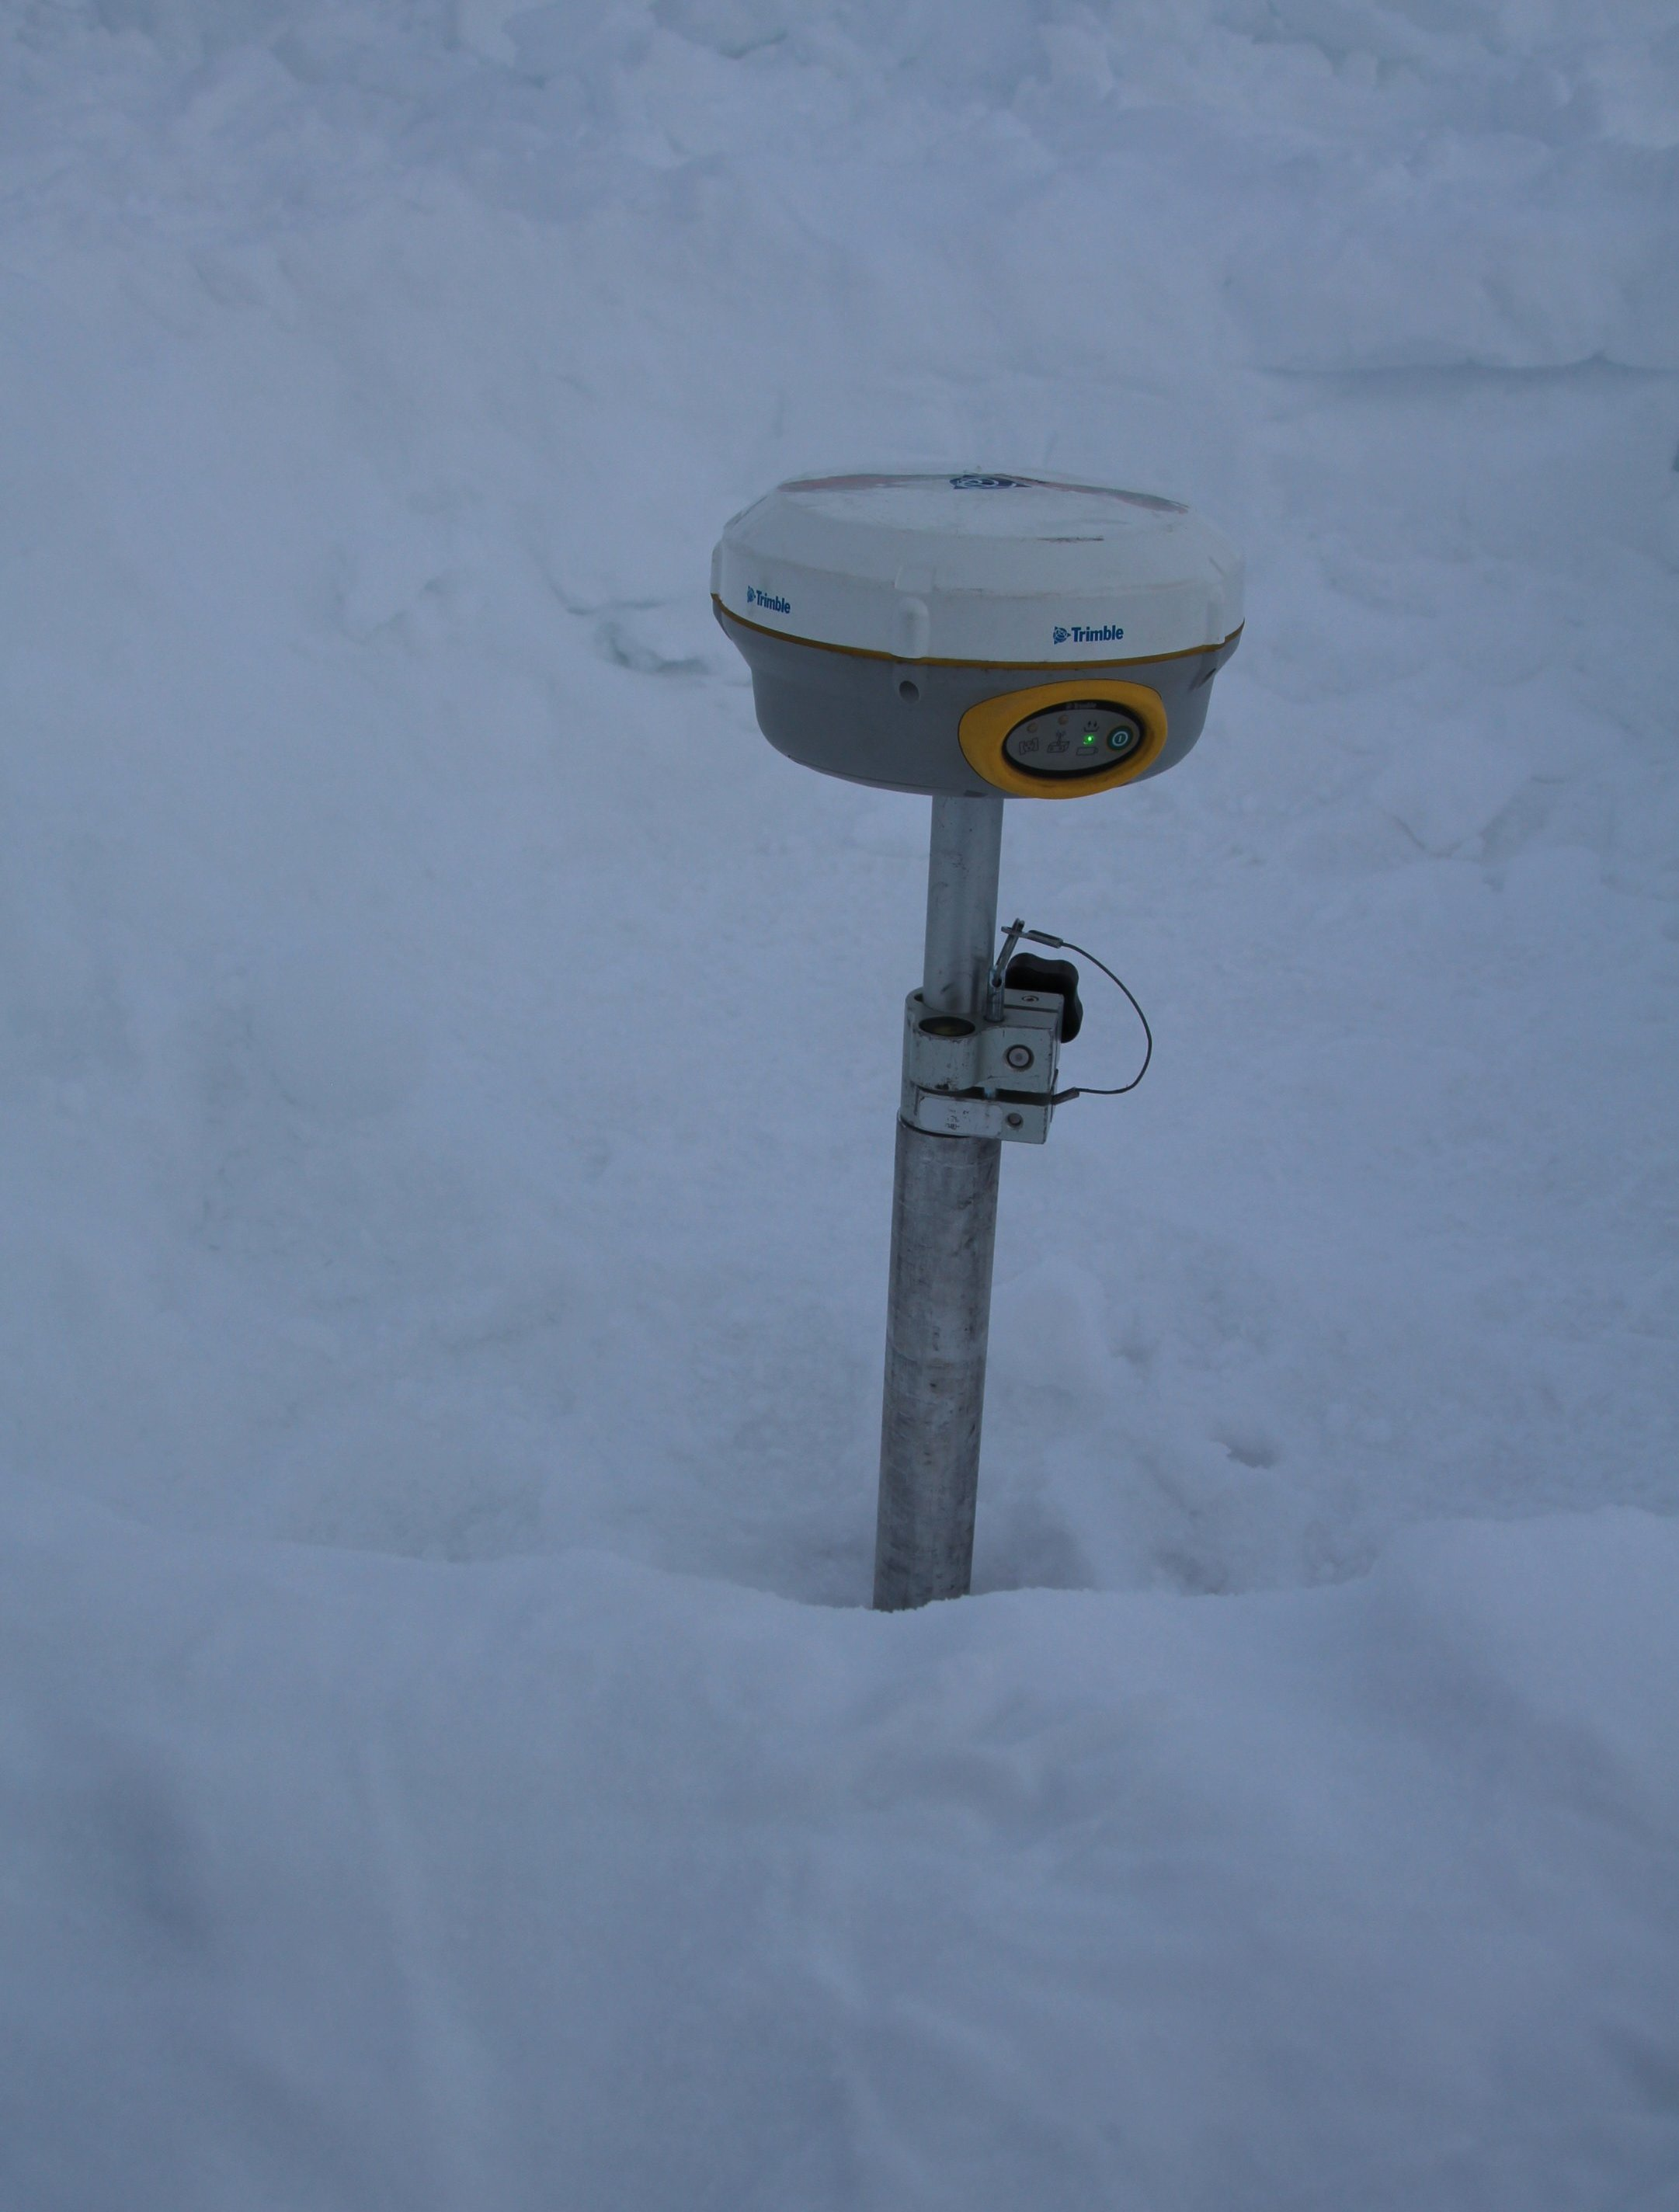
\includegraphics[width=0.485\linewidth]{/figs/pictures/setup_ontop.JPG}
\caption{Setup while the GPS measurement next to the stake (left) and on top of the stake (right).}
\end{figure}
